% ----  added separate section for the ratio method

As for the energy reconstruction, in the ratio method the time of a rechit in an ECAL crystal is estimated from the ten consecutively sampled pulse amplitudes that are recorded every 25 ns. The ratio of any two consecutive amplitudes, sampled from a signal with the expected pulse shape, uniquely determines the timing of an isolated pulse measured in a particular crystal, relative to the LHC beam clock. In Figure~\ref{tec_pulseratio}, the ratio, $R$, of two consecutively measured amplitudes, $A(T)$ and $A(T+25 ns)$, is shown as a function of the time difference $T-T_{max}$, where $T_{max}$ is defined as the time when the pulse reaches its maximum value. The first three measured pulse heights, $A(1)$, $A(2)$, and $A(3)$ are typically used to measure the pedestal values ( measured amplitude corresponding to "zero" ) for the pulse. Ratios for $R(A(4)/A(5))$ through $R(A(7)/A(8))$ are used to estimate the pulse timing. Since the remaining ratios arising from the tail of the pulse are insensitive to the pulse timing, they are not utilized. The rechit time for a pulse in a crystal is determined from the weighted averages of three consecutive values of $R(A(4)/A(5))$ through $R(A(7)/A(8))$.

The clock distribution system has its own delays relative to the actual collision time and these delays vary from crystal to crystal. To compensate for this the timing is calibrated using actual prompt relativistic particles so that the mean reconstructed time, per channel, is defined to be zero \cite{CMS-PAS-EXO-19-005}.

\begin{figure}[htbp]
\begin{center}
\resizebox{0.7\linewidth}{!}{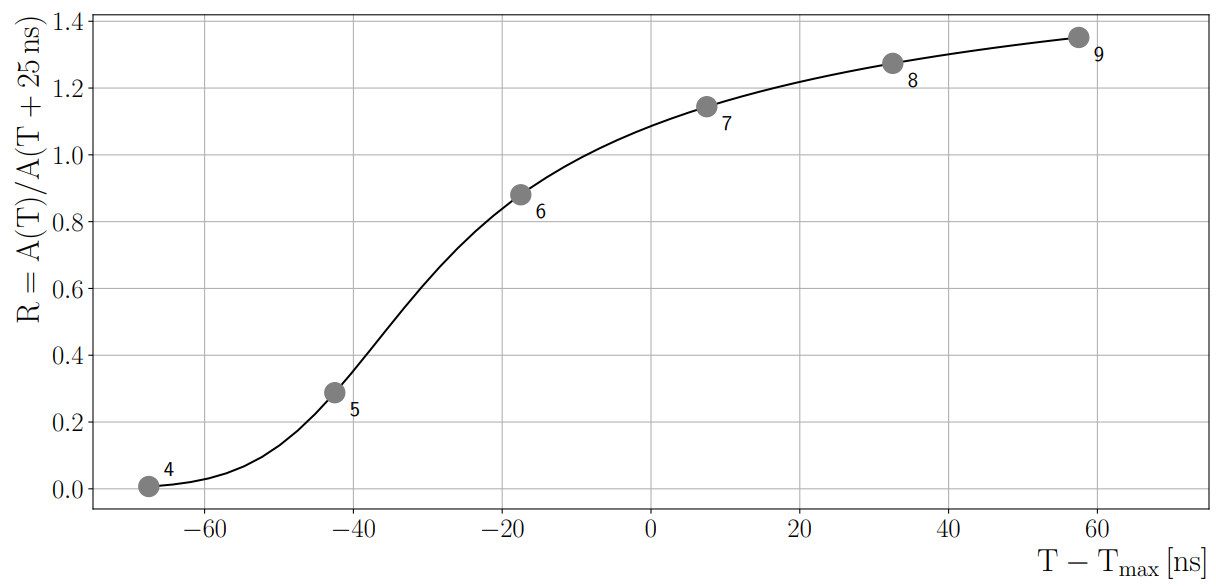
\includegraphics{fig/sec_reco/ratio_tvR_mod.png}}
\caption{The ratio, $R$, of two consecutively measured amplitudes, $A(T)$ and $A(T+25 ns)$, as a function of the time difference $T-T_{max}$, where $T_{max}$ is the time when the pulse reaches its maximum value. The first three amplitudes, $A(1)$, $A(2)$, and $A(3)$, typically used to measure the pedestals values for the pulse, are not used. The rechit time is determined from the weighted averages of three consecutive value of $R(A(4)/A(5))$ through $R(A(7)/A(8))$.}
\label{tec_pulseratio}
\end{center}
\end{figure}

\begin{equation}\label{ratio_eqt}
t_{ECAL} = \sum_{t} \frac{t^{i}_{ECAL}}{\sigma^{2}_{i}}/\sum_{t} \frac{1}{\sigma^{2}_{i}}\qquad
\end{equation}

The time of arrival for a reconstructed particle at the ECAL, $t_{ECAL}$ in Equation~\ref{ratio_eqt}, is calculated based on a weighted sum of the reconstructed times in each of the ECAL crystals that compromises the cluster of crystals associated with the reconstructed particle. In this equation $t^{i}_{ECAL}$ is the pulse time in crystal $i$. $\sigma_{i}$ is the estimated time resolution of the signal pulse in crystal $i$. The time resolution weights $\sigma^{2}_{i}$ are estimated based on the intrinsic time resolution of the ECAL crystal sensors \cite{Collaboration_2010}. 

The ratio method assumes that the sampled signal pulse is well isolated in time.  In the higher PU environments of Run 2 and Run 3 this is no longer a good assumption. As was previously noted, for Run 2 and beyond, the observed pulse shape of a signal in an ECAL channel is a superposition of a nominal, or in-time, pulse that is of interest and multiple, non-negligible, out-of-time (OOT) pulses. This situation is illustrated in Figure~\ref{tec_multifit2} with a single OOT pulse for clarity. The resultant superposition of multiple pulses into a single sampled pulse shape is not well modeled by the expected pulse shape as measured in the pulse shape templates. In the case where the "sampled" pulse shape differs significantly from the pulse shape template, the ratio of any two consecutive amplitudes will not uniquely determine the timing of the pulse measured in a crystal.
